 \documentclass[11pt]{article}

\usepackage{amsmath}
\usepackage{amssymb}
\usepackage{amsthm}
\usepackage{marvosym}
\usepackage{wasysym}
\usepackage{mathdots}
\usepackage{mathrsfs}
\usepackage{setspace}
\usepackage{graphics}
\usepackage{enumitem}
\usepackage[margin=1.2in]{geometry}
%\usepackage{fancyvrb}
%\usepackage{xcolor}
%\usepackage{biblatex}

%\usepackage{pdfsync}
%\usepackage{remark,subeqnarray,mc,epsf}
%\usepackage[notcite,notref]{showkeys}
\usepackage[active]{srcltx}
\usepackage{graphicx,color}
\usepackage[table]{xcolor}

% \usepackage{A4wide}
% \usepackage[active]{srcltx}
\usepackage{graphicx,color}%psfrag

\newtheorem{Theorem}{{\bf Theorem}}[section]
\newtheorem{Lemma}{{\bf Lemma}}[section]

\newcommand{\sA}{{\mathcal A}}
\newcommand{\sB}{{\mathcal B}}
\newcommand{\sC}{{\mathcal C}}
\newcommand{\sD}{{\mathcal D}}
\newcommand{\sE}{{\mathcal E}}
\newcommand{\sF}{{\mathcal F}}
\newcommand{\sG}{{\mathcal G}}
\newcommand{\sH}{{\mathcal H}}
\newcommand{\sI}{{\mathcal I}}
\newcommand{\sK}{{\mathcal K}}
\newcommand{\sL}{{\mathcal L}}
\newcommand{\sM}{{\mathcal M}}
\newcommand{\sN}{{\mathcal N}}
\newcommand{\sP}{{\mathcal P}}
\newcommand{\sR}{{\mathcal R}}
\newcommand{\sU}{{\mathcal U}}
\newcommand{\sV}{{\mathcal V}}
\newcommand{\sW}{{\mathcal W}}
\newcommand{\sX}{{\mathcal X}}
\newcommand{\sY}{{\mathcal Y}}
\newcommand{\sZ}{{\mathcal Z}}

\newcommand{\cD}{{\mathfrak D}}
\newcommand{\cF}{{\mathfrak F}}
\newcommand{\cH}{{\mathfrak H}}
\newcommand{\cS}{{\mathfrak S}}
\newcommand{\cd}{{\mathfrak d}}
\newcommand{\sign}{\text{sign}}

\newcommand{\nn}{\nonumber}

\newcommand{\Lat}{\mbox{Lat}}
\newcommand{\ran }{{\mbox{ran\,}}}

%%%%%%%%%%%%%%%%%%%%%%%%%%%%%%%%%%%%%
\def\a{{\alpha}}
\def\b{\beta}
\def\c{\gamma}
\def\d{\delta}
\def\de{\Delta}
\def\e{\eta}
\def\g{\gamma}
\def\ga{\Gamma}
\def\k{\kappa}
\def\l{\lambda}
\def\la{\Lambda}
\def\s{\sigma}
\def\si{\Sigma}
\def\t{\tau}
\def\o{\omega}
\def\om{\Omega}
\def\th{\theta}
\def\tht{\Theta}
\def\va{\varphi}
\def\vp{\varepsilon}
\def\vt{\vartheta}
\def\z{\zeta}
\def\ts{\times}
\def\gap{{\textrm{gap}\,}}
\def\iy{\infty}
\def\im{{\rm Im\, }}
\def\codim{{\textrm{codim}\,}}
\def\kr{{\rm Ker\, }}
\def\diag{{\textrm{diag}\, }}
\def\degr{{\textrm{degree}\, }}
\def\ds{\,\textup{d}s\, }
\def\dr{\,\textup{d}r\, }
\def\dt{\,\textup{d}t\, }
\def\du{\,\textup{d}u\, }
\def\dl{\,\textup{d}\lambda\, }
\def\dmu{\,\textup{d}\mu\, }
\def\dtau{\,\textup{d}\tau\, }
\def\ra{{\textrm{Range}\, }}
\def\rank{{\textrm{rank}\, }}
\def\pol{{\textrm{Pol}\,}}
\def\ind{{\textrm{ind}\,}}
\def\pr{{\textrm{pr}\, }}
\def\col{{\textrm{col}}}
\def\row{{\textrm{row}\, }}
\def\lg{\langle}
\def\rg{\rangle}
\def\wh{\widehat}
\def\wt{\widetilde}
\def\ol{\overline}
\def\ul{\underline}
\def\dia{\nabla}

%% \newcommand{\bOm}{{\boldsymbol\Omega}}  gaf beta Om aan elkaar. Dat wilde ik niet.

\def\BC{{\mathbb C}}
\def\BD{{\mathbb D}}
\def\BN{{\mathbb N}}
\def\BP{{\mathbb P}}
\def\BQ{{\mathbb Q}}
\def\BR{{\mathbb R}}
\def\BT{{\mathbb T}}
\def\BZ{{\mathbb Z}}


%%\def\pos{\textup{\tiny{+}}}

% \def\sp{\textrm{\tiny{\textrm{+}}}}

%%%%%%%%%%%%%%%%%%%%%%%
\renewcommand{\theequation}{\arabic{section}.\arabic{equation}}
\newcommand{\eq}{\addtocounter{equation}{1}(\theequation)}
%%%%%%%%%%%%%%%%%%%%%%%


\newcommand{\bpr}{{\noindent\textbf{Proof.}\ \ }}
\newcommand{\epr}{{$\mbox{\ }$ \hfill $\Box$}}

\newtheorem{thm}{Theorem}[section]
\newtheorem{prop}[thm]{Proposition}
\newtheorem{proposition}[thm]{Proposition}
\newtheorem{lem}[thm]{Lemma}
\newtheorem{lemma}[thm]{Lemma}
\newtheorem{cor}[thm]{Corollary}
\newtheorem{corollary}[thm]{Corollary}
\newtheorem{rem}[thm]{Remark}
\newtheorem{remark}[thm]{Remark}
\newtheorem{definition}[thm]{Definition}
\newtheorem{exa}[thm]{Example}
\newtheorem{probl}[thm]{Problem}
\newtheorem{theorem}{Theorem}[section]

\newcommand{\ands}{\quad\mbox{and}\quad}
\newcommand{\spe}{{\textup{sp}}}

\newcommand{\bvec}{\textup{\textbf{vec}}\,}
\newcommand{\brow}{\textup{\textbf{row}}}

\newcommand{\supp}{\textup{supp\,}}
\newcommand{\rad}{ r_{\textup{spec}}}

\definecolor{purple}{rgb}{.6,0,.7}
\newcommand{\tcp}{\textcolor{purple}}
\newcommand{\tcb}{\textcolor{blue}}
\definecolor{green}{rgb}{.0,.6,.0}
\newcommand{\tcg}{\textcolor{green}}
\newcommand{\tcr}{\textcolor{red}}

\newcommand{\bL}{\textup{\textbf{L}}}
\newcommand{\bT}{\textup{\textbf{T}}}
\newcommand{\bH}{\textup{\textbf{H}}}
\newcommand{\bI}{\textup{\textbf{I}}}
\newcommand{\bP}{\textup{\textbf{P}}}
\newcommand{\bR}{\textup{\textbf{R}}}
\newcommand{\bZ}{\textup{\textbf{Z}}}

\newcommand{\Rat}{\textup{Rat}}


\newcommand{\tH}{\tilde{H}}
\newcommand{\tT}{\tilde{T}}
\newcommand{\tL}{\tilde{L}}
\newcommand{\tR}{\tilde{R}}

\addcontentsline{toc}{section}{text_to_be_added}

\date{}

\author{}


\begin{document}
\title{ {\bf   Lab 6:  The 2 DOF Helicopter.  (Answer Sheet)\footnote{Part of this write up and Figures were
taken directly from Quanser's lab manuals; Quanser Inc.} \\



\vspace{1in}
Name: Rajan Phadnis  }}

\maketitle

\newpage

\vspace{1 cm}
\textcolor{blue}{\noindent{\huge{ $\mathfrak{Prelab \,\,1}$}}}
\medskip

Recall that our feedback system is given by

\begin{equation*}
     \dot{x}=(A-BK)x+BNr\quad \mbox{and} \quad y=C x
\end{equation*}.

% Use Matlab to find the transfer function of the controlled system.
Now show that, for $A-BK$ stable, under a constant input voltage $r=\begin{bmatrix} \theta_d & \psi_d \end{bmatrix}^{tr}$ (where $tr$ denotes the transpose), and a scale input factor $N=-(C(A-BK)^{-1}B)^{-1}$, the controlled system satisfies 

\begin{equation*}
x(\infty)=\lim_{t\to\infty} x(t)= \lim_{t\to\infty}  \begin{bmatrix} \theta(t) \cr \psi(t)) \cr \dot{\theta}(t) \cr \dot{\psi}(t) \end{bmatrix}= \begin{bmatrix} \theta_d \cr \psi_d \cr 0 \cr 0 \end{bmatrix}.  
\end{equation*}

Hint: One can approach this by using the Final Value Theorem. Another method is to notice that in steady-state $\dot{x}=0$ and $0=A-BKx(\infty)+BNr$.

(3 points)

\[(A-BK)x+BNr=0\]

solve for x:

\[x=-BNr[A-BK]^{-1}\]

Substitute N and pull out C

\[Cx=-B(A-BK)^{-1}-((A-BK)^{-1}B)^{-1}r\]

Take the limit of the new $Cx$ expression and put into matrix form to solve/simplify:

\[Cx(\infty) = r\]

\[\begin{bmatrix}
    $1$ & $0$ & $0$ & $0$\\
    $0$ & $1$ & $0$ & $0$\end{bmatrix}\cdot\begin{bmatrix}
        \theta_d\\
        \psi_d\\
        $0$\\
        $0$
    \end{bmatrix}=r=\begin{bmatrix}
        \theta_d\\
        \psi_d
    \end{bmatrix}\]

So, yes, under those conditions, the controlled system satisfies that system of equations.

\newpage
\textcolor{blue}{\noindent{\huge{  $\mathfrak{Prelab \,\,2}$}}}
\medskip

Using pole placement or LQR, design a controller to make the helicopter track a square wave both in pitch and yaw (remember there are two inputs and two outputs now). Simulate the helicopter's behavior under your controller using lsim. (3 points) To do so perform the following steps:

\medskip

\begin{enumerate}

    \item Open and load the Aero 2 parameters given in aero2\_parameters\_helicopter.m
     \item Use Matlab to determine the system's controllability
     
    \item Calculate your gain matrix $K$ using pole placement or LQR.
    
    \item Now create two vectors corresponding to a \textit{square} wave. The first needs to have an amplitude of  20$^o$ and a frequency of 0.05 Hz (pitch) and the second an amplitude to 60$^o$ and a frequency of 0.04 Hz (yaw).

        \item Use Matlab's \textbf{ss} and \textbf{ss2tf} and  \textbf{lsim} functions to simulate the system (remember we have 2 inputs now). 
   

    \item Optimize your controller by comparing the simulation to the reference and changing $K$ accordingly.
    \item Give your best $K$ and mention whether you used pole placement or LQR. If you used pole placement give the poles you selected. If you used LQR, give the Q and R matrices. Explain why you selected one method or the other.
    \item Plot the system's response to your best controller both in pitch and yaw.

\end{enumerate}

\textbf{Best \( K \)= }\\

\[
\begin{bmatrix}
    $4427.7$ & $-670.4$ & $798.4$ & $-151.4$\\
    $2487.5$ & $2802.3$ & $432.9$ & $462.1$\\
\end{bmatrix}
\]

\textbf{LQR or Pole Placement?}\\

Pole placement

\vspace{1cm} % Space for the answer

\textbf{Poles or \( Q \) and \( R \) matrices\\}

Poles: [-10, -11, -12, -13]

\vspace{0.5cm} % Space for the answer

\textbf{Justification for Method Choice:}\\

Pole placement was the easiest to implement, given that I could easily get the state-space version of the tf, then convert that to a tf pretty easily. 
\vspace{2cm} % Space for the explanation

\textbf{Plots for the system's response in pitch and yaw:}\\

    \centering
  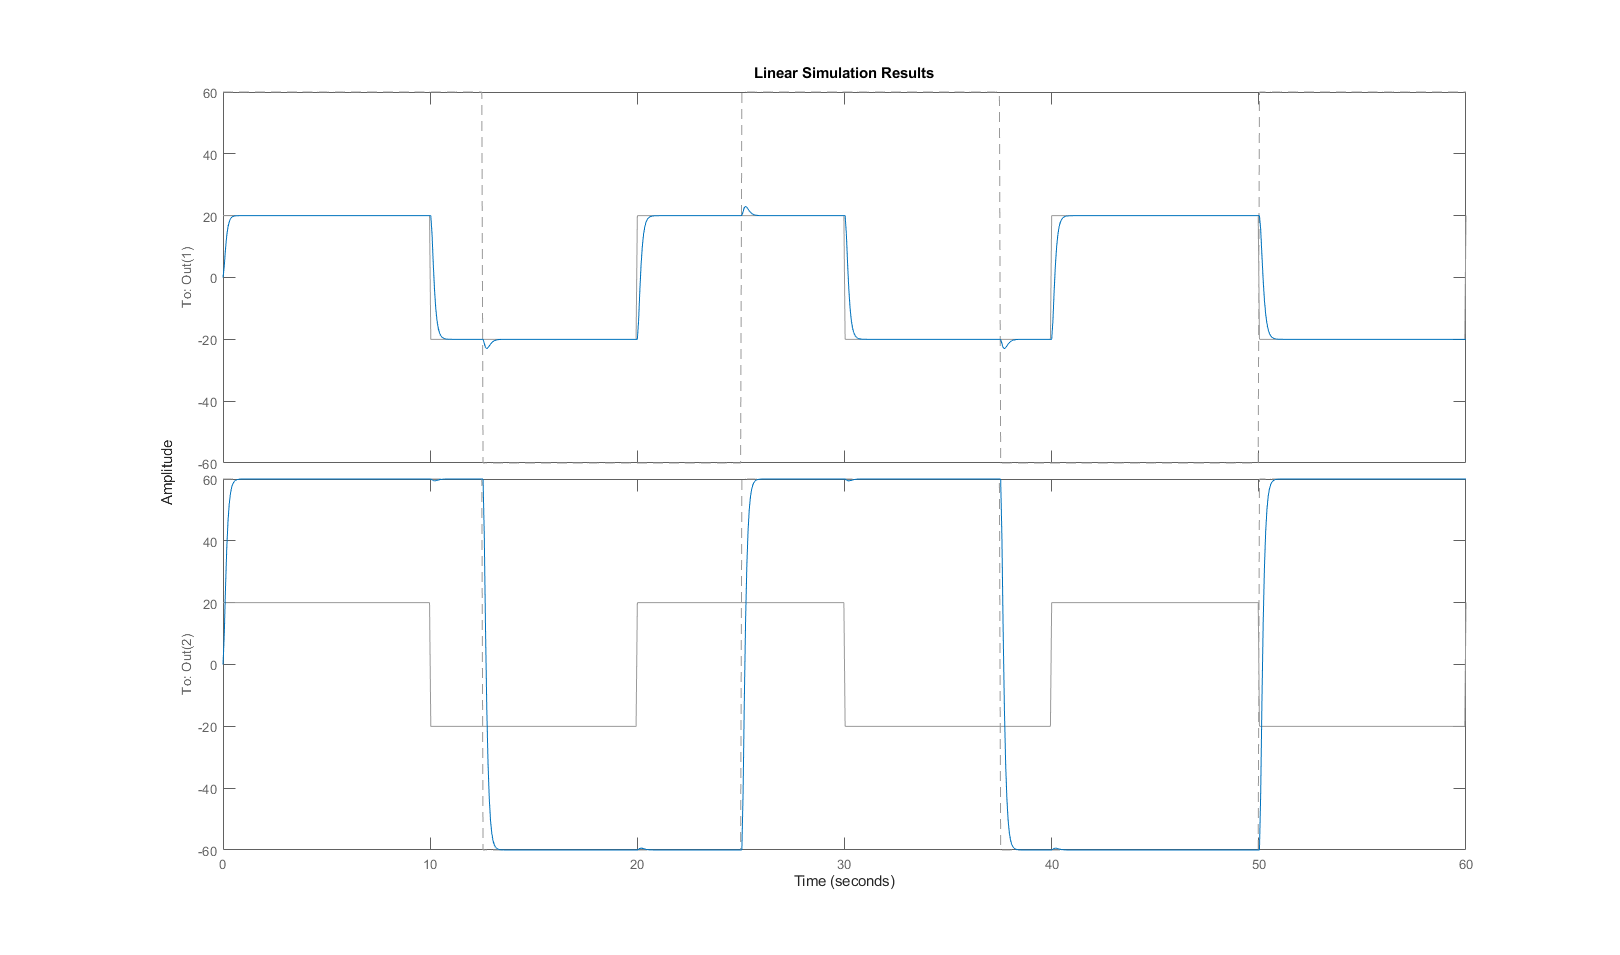
\includegraphics[width=5in]{prelab2.png}


\begin{figure}[ht!]
  \centering
  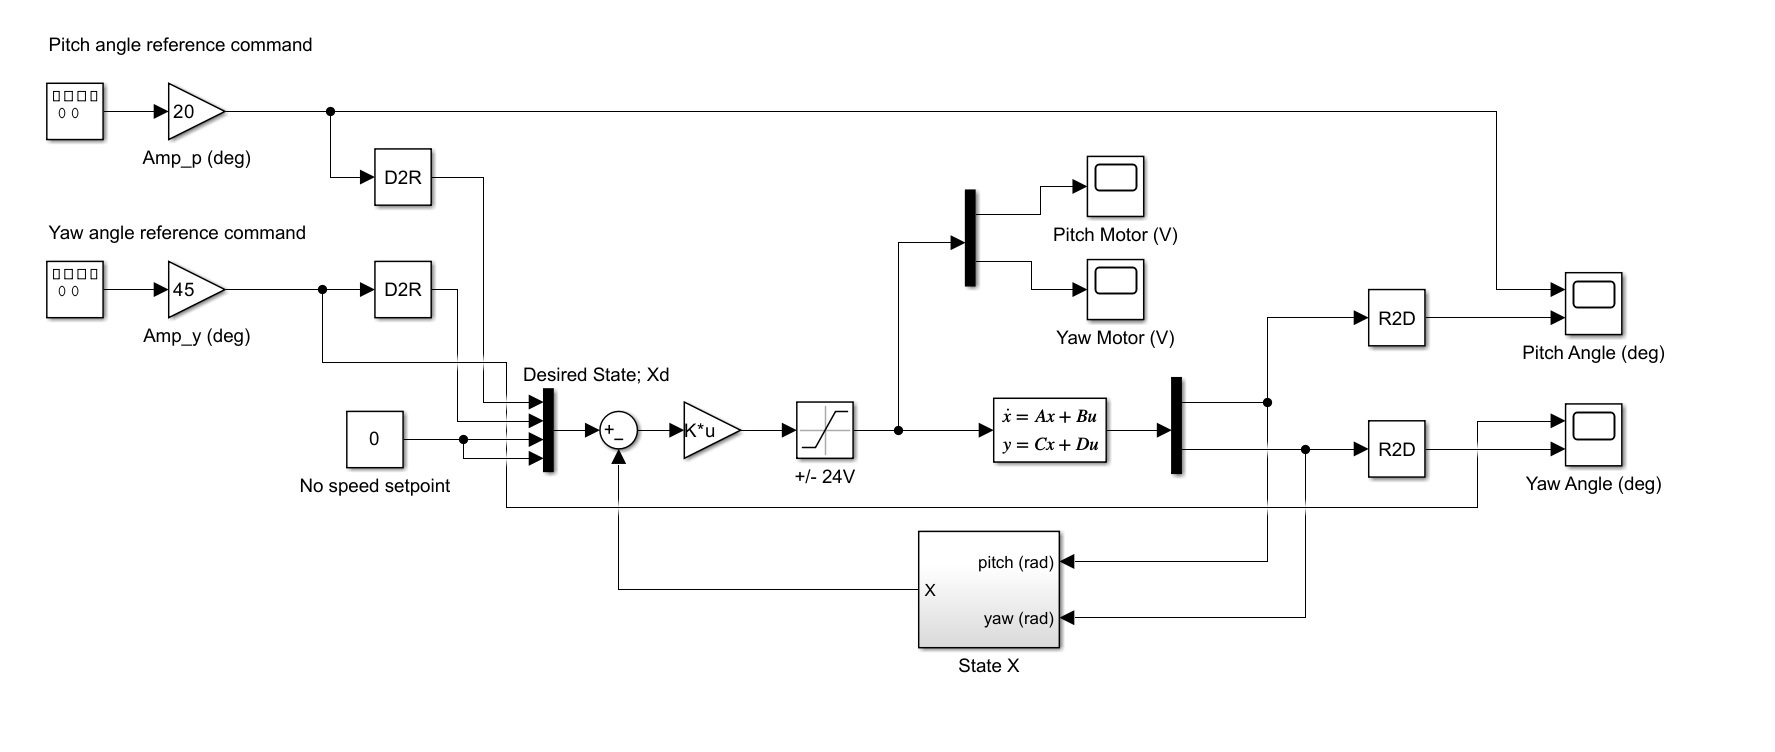
\includegraphics[width=5in]{simulink_s.jpg}
  \caption{Simulink model for simulated the controlled response of the Aero 2.}
  \label{fig:simulinks}
\end{figure}



\newpage

\textcolor{blue}{\noindent{\huge{  $\mathfrak{Prelab \,\,3}$}}}
\medskip

Design a trace function to map your art onto the xy plane, this can be achieved by discrete functions or continuous functions such as a Fourier series or parametric functions. Plot the function in the xy coordinates. Now implement a second function that takes your xy plane coordinates and transforms them into pitch and yaw angles (think spherical coordinates). Plot your new transformed input function.  (4 points)

\centering
  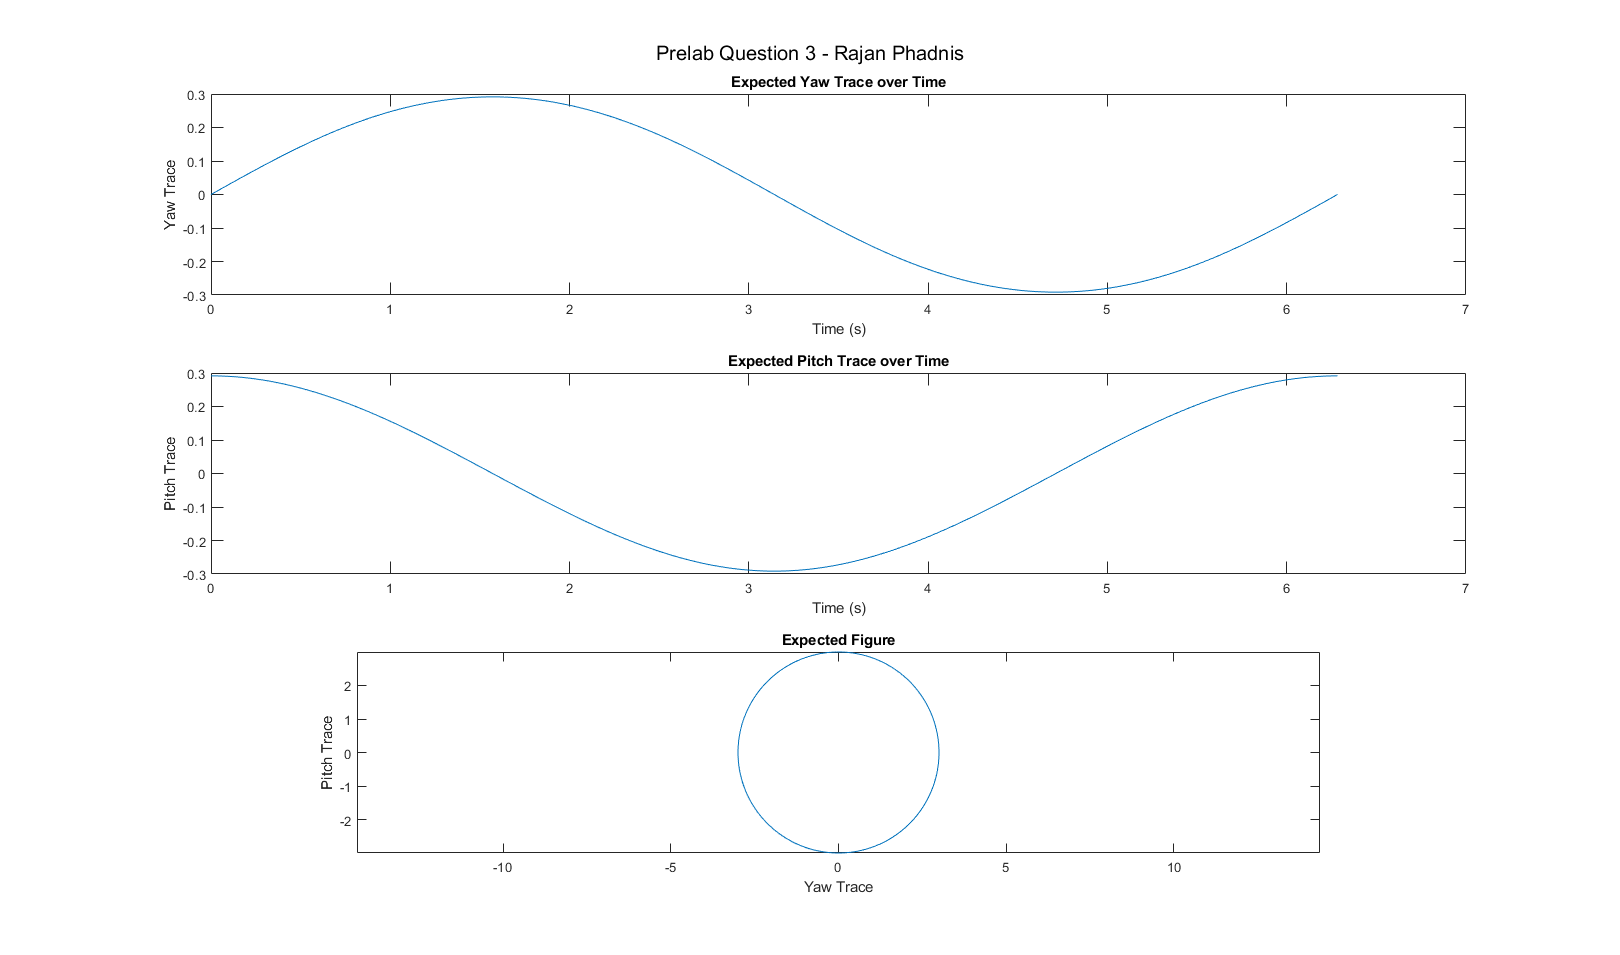
\includegraphics[width=6.5in]{prelab3.png}

\newpage

\noindent \textcolor{red}{{\huge  Experiment 1}}
\vspace{0.5 cm}

Test your controllers on the Aero 2 in helicopter configuration.
\vspace{0.5 cm}

\medskip

To run this experiment
\begin{enumerate}

\item Set the Aero 2 in helicopter configuration. To do so, lock the yaw using the appropriate knob. Now unlock the pitch and carefully move the weights to balance the helicopter (see Lab Write-up). At rest, it should be parallel to the ground. Once the helicopter is well-balanced you can unlock the yaw again.

  \item Open and load the Aero 2 parameters given in aero2\_parameters\_helicopter.m
    \item Open q\_aero2\_2dof\_lqr\_control.slx
       This model should look like the QUARC-Simulink model in Figure \ref{fig:simulinkq}.
         \item Set the waveform in both signal generators to \textit{square}. Change the pitch amplitude to 20$^o$ and the yaw amplitude to 60$^o$.

  \item Starting with the helicopter parallel to the ground, run the Simulink model for 60 seconds using the controller $K$ you designed.
    \item Optimize your controller by comparing the helicopter's motion to the reference and changing $K$ accordingly.
    \item Give your best $K$ and mention whether you used pole placement or LQR. If you used pole placement give the poles you selected. If you used LQR, give the Q and R matrices. (20 points) \vspace{0.5 cm}\textbf{Best \( K \)=}\\
\vspace{2cm} % Space for the answer

\textbf{LQR or Pole Placement?}\\

\vspace{1cm} % Space for the answer

\textbf{Poles or \( Q \) and \( R \) matrices\\}

\vspace{1cm} % Space for the answer


\newpage
    
    \item Plot the system's response to your best controller both in pitch and yaw. (20 points)
    \vspace{9 cm}
    
     \item Repeat the procedure but now use a \textit{sine} waveform in both signal generators. Give your best K, poles or Q and R, and include the corresponding plots. (30 points)

\newpage

    

    \vspace{7 cm}
    
    
\end{enumerate}


\begin{figure}[ht!]
  \centering
  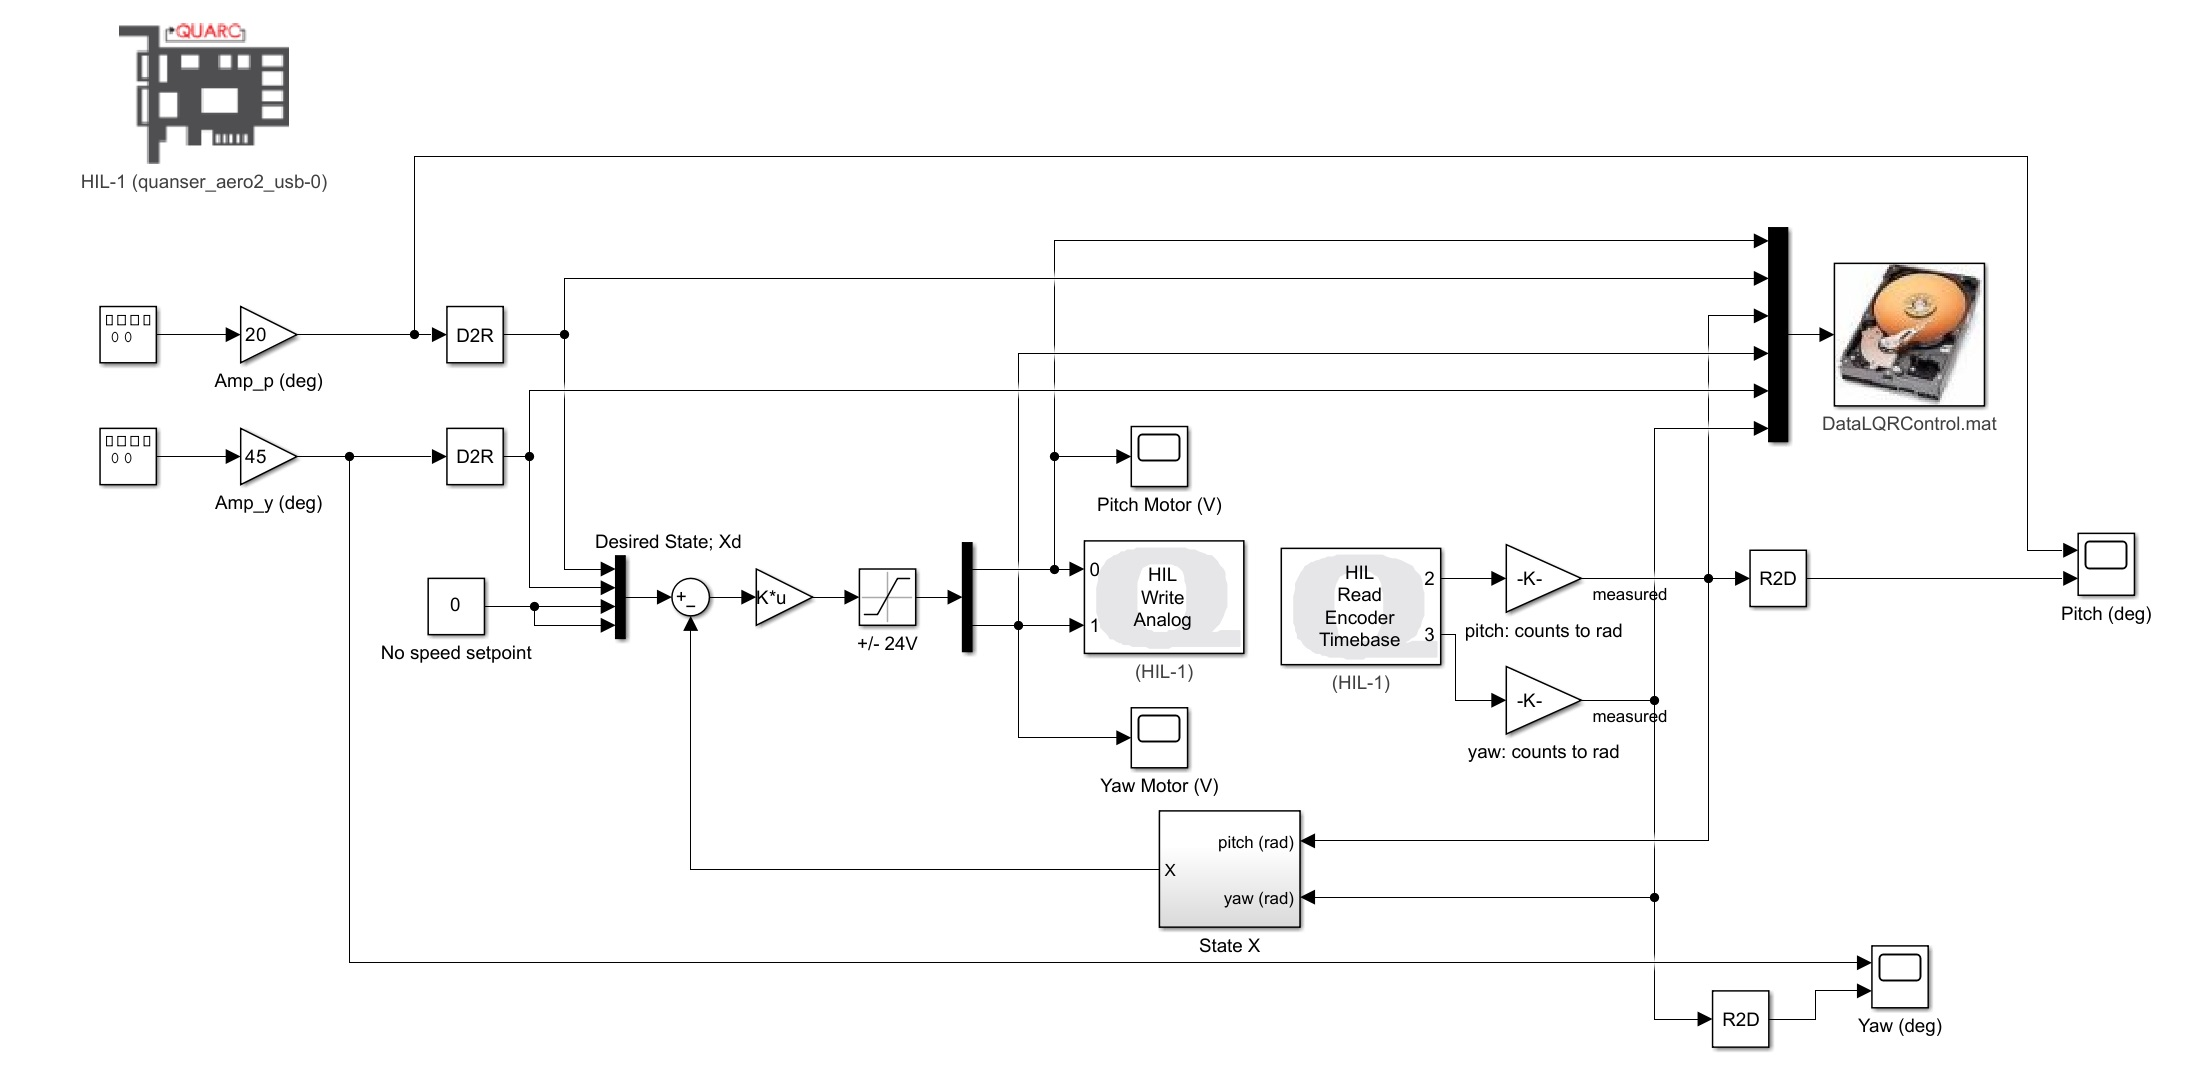
\includegraphics[width=5in]{simulink_q.jpg}
  \caption{QUARC-Simulink model for controlling the Aero 2.}
  \label{fig:simulinkq}
\end{figure}


\noindent \textcolor{red}{{\huge  Experiment 2}}
\vspace{0.5 cm}

\begin{enumerate}
    \item Replace the input signal in the Quanser Simulink model 'q\_aero2\_2dof\_lqr\_control\_customsignal.slx' to plot a square or a rectangle

    \item Compute an initial K using LQR and the integral model to make the helicopter follow the square or rectangle.

     \item Optimize your gain matrix K and try to improve the performance of the integral controller (use the system matrices given above).  State whether you used LQR or pole placement. Give your best K eigenvalues or Q and R. (15 points)
    
    \item Now replace the input signal with your drawing and watch the art come to life. 

    \item Optimize your gain matrix further K.    
    
    \item Plot the artwork using the pitch and yaw measurements obtained in the previous step and compare it to the original input artwork, describe any differences you observed, and in a couple of lines explain what would be the steps to resolve these differences.

    \item Once you are satisfied with your results send your functions, signal, and K matrix to the TA so we can test them with the actual laser.
   
    \item Include a picture of your best artwork. (5 points)
\end{enumerate}


Note: Although the laser is low-powered, we will take standard laser-safety measures. The laser setup will be operated only after all teams submit their functions and best K. We ask you to please stand while the laser is in use to prevent any potential eye exposure (direct or through reflections).

\vspace{1cm}

 \textbf{Best \( K \)=}\\
\vspace{1cm} % Space for the answer

\textbf{LQR or Pole Placement?}\\

\vspace{0.5 cm} % Space for the answer

\textbf{Poles or \( Q \) and \( R \) matrices\\}

\vspace{2cm} % Space for the answer


\clearpage


\textbf{Add a picture of your artwork below.}\\

  \end{document}
